% Use only LaTeX2e, calling the article.cls class and 12-point type.
\documentclass[12pt]{article}

% Users of the {thebibliography} environment or BibTeX should use the
% scicite.sty package, downloadable from *Science* at
% www.sciencemag.org/about/authors/prep/TeX_help/ .
% This package should properly format in-text
% reference calls and reference-list numbers.

% Science template required packages
\usepackage{scicite}

\usepackage{times}

% add-ons for rticles
% based on arxiv.sty
\usepackage[utf8]{inputenc} % allow utf-8 input
\usepackage[T1]{fontenc}    % use 8-bit T1 fonts
\usepackage[hidelinks]{hyperref}       % hyperlinks
\usepackage{url}            % simple URL typesetting
\usepackage{booktabs}       % professional-quality tables
\usepackage{amsfonts}       % blackboard math symbols
\usepackage{nicefrac}       % compact symbols for 1/2, etc.
\usepackage{microtype}      % microtypography
\usepackage{lipsum}
\usepackage{graphicx}

% the basics
\usepackage{amsmath}
\usepackage{calc}
\usepackage{tabularx}

% for figure adjustment
\usepackage{placeins}
\usepackage{flafter}




% tightlist command for lists without linebreak
\providecommand{\tightlist}{%
  \setlength{\itemsep}{0pt}\setlength{\parskip}{0pt}}

% From pandoc table feature
\usepackage{longtable,booktabs,array}
\usepackage{calc} % for calculating minipage widths
% Correct order of tables after \paragraph or \subparagraph
\usepackage{etoolbox}
\makeatletter
\patchcmd\longtable{\par}{\if@noskipsec\mbox{}\fi\par}{}{}
\makeatother
% Allow footnotes in longtable head/foot
\IfFileExists{footnotehyper.sty}{\usepackage{footnotehyper}}{\usepackage{footnote}}
\makesavenoteenv{longtable}

% Pandoc citation processing



% The following parameters seem to provide a reasonable page setup.

\topmargin 0.0cm
\oddsidemargin 0.2cm
\textwidth 16cm
\textheight 21cm
\footskip 1.0cm


%The next command sets up an environment for the abstract to your paper.
\usepackage{setspace}

\newenvironment{sciabstract}{%
\begin{quote} \singlespacing}
{\end{quote}}


% If your reference list includes text notes as well as references,
% include the following line; otherwise, comment it out.

\renewcommand\refname{References and Notes}

% The following lines set up an environment for the last note in the
% reference list, which commonly includes acknowledgments of funding,
% help, etc.  It's intended for users of BibTeX or the {thebibliography}
% environment.  Users who are hand-coding their references at the end
% using a list environment such as {enumerate} can simply add another
% item at the end, and it will be numbered automatically.

\newcounter{lastnote}
\newenvironment{scilastnote}{%
\setcounter{lastnote}{\value{enumiv}}%
\addtocounter{lastnote}{+1}%
\begin{list}%
{\arabic{lastnote}.}
{\setlength{\leftmargin}{.22in}}
{\setlength{\labelsep}{.5em}}}
{\end{list}}


% Include your paper's title here

\title{\bf Mainstreaming Race Science}


% Place the author information here.  Please hand-code the contact
% information and notecalls; do *not* use \footnote commands.  Let the
% author contact information appear immediately below the author names
% as shown.  We would also prefer that you don't change the type-size
% settings shown here.


\author{
Daniel J. Hicks,\textsuperscript{*}
and Emilio Lobato
\\\textsuperscript{*}Corresponding author: Daniel J. Hicks, \href{mailto:dhicks4@ucmerced.edu}{\nolinkurl{dhicks4@ucmerced.edu}}.
}

% Include the date command, but leave its argument blank.

\date{}



%%%%%%%%%%%%%%%%% END OF PREAMBLE %%%%%%%%%%%%%%%%



\begin{document}
\maketitle
\section*{Supplementary Text}
\renewcommand{\thesection}{S\arabic{section}}
\hypertarget{materials-and-methods}{%
\section*{Materials and methods}\label{materials-and-methods}}

\hypertarget{corpus-assembly}{%
\subsection*{Corpus assembly}\label{corpus-assembly}}

\begin{figure}
\centering
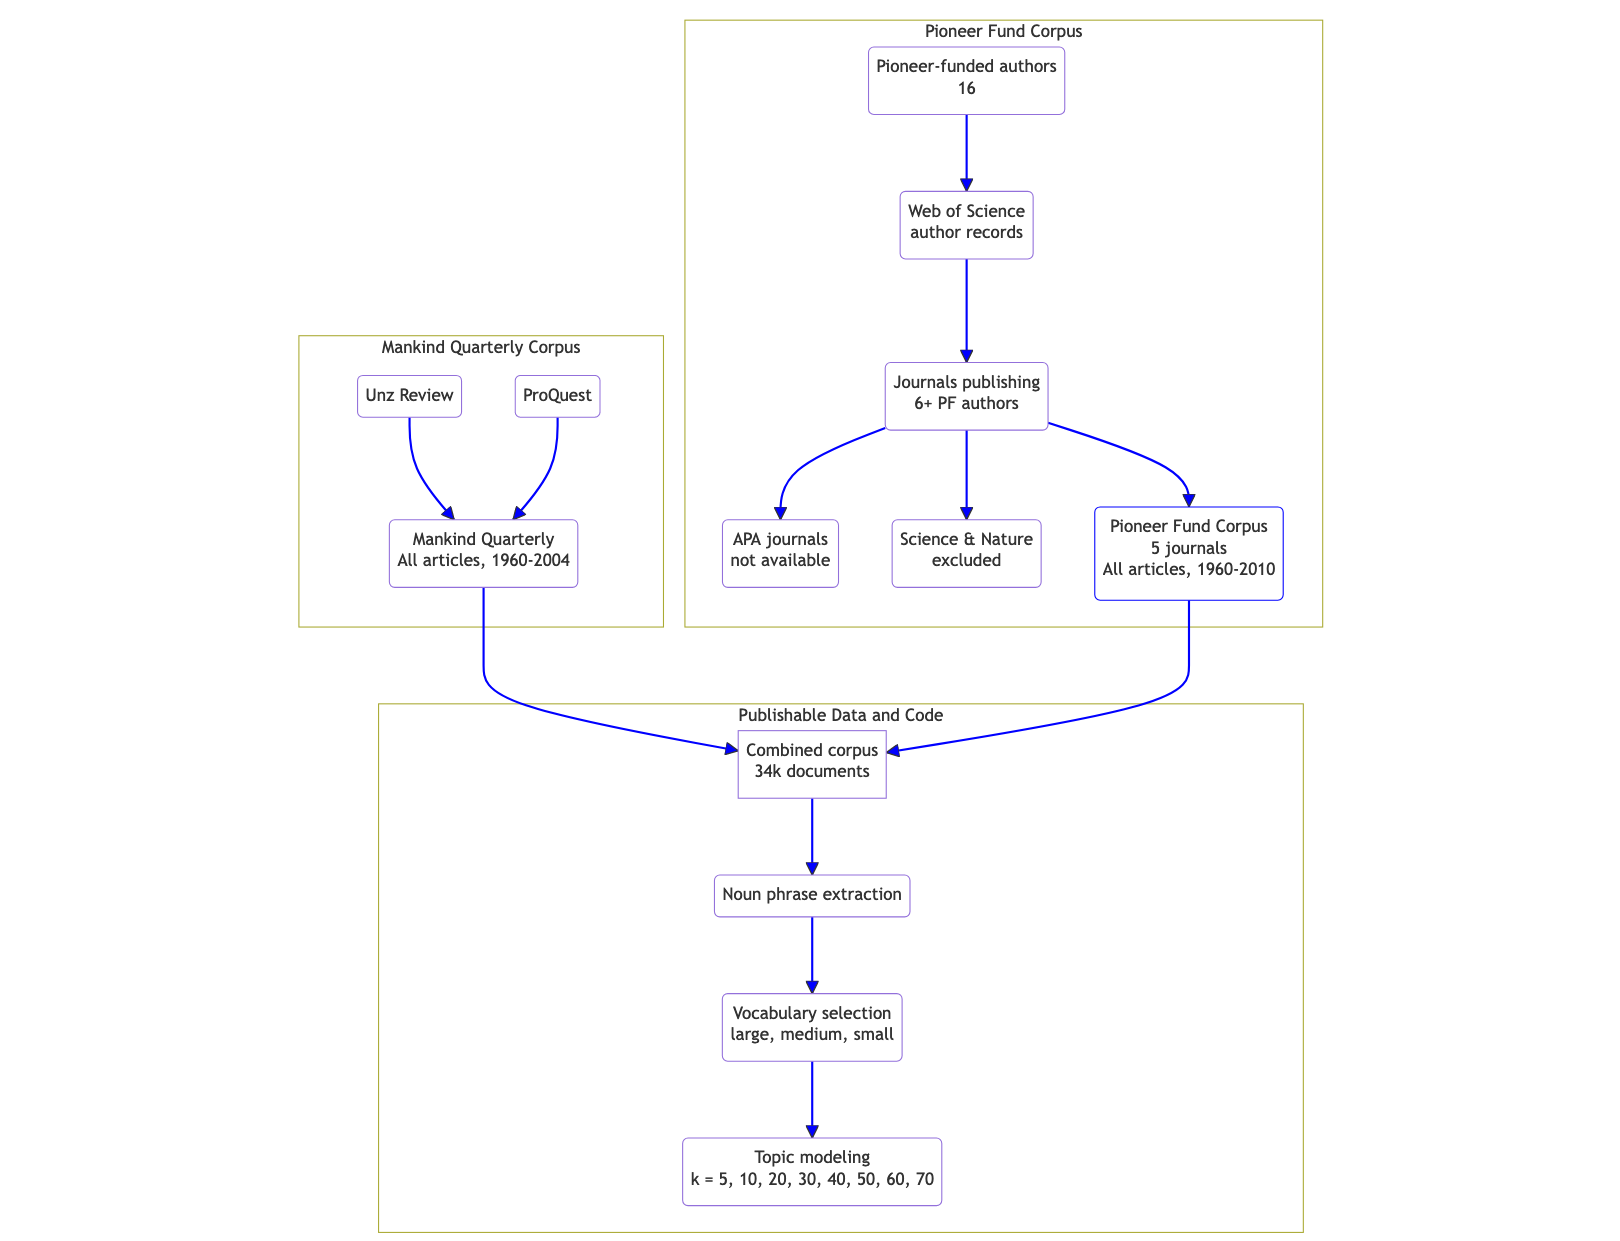
\includegraphics[width=8in,height=6.1in]{img/dataset.png}
\caption{Corpus assembly. (\#fig:corpus)}
\end{figure}

Corpus assembly is summarized in figure @ref(fig:corpus). The corpus was assembled in two parts, one for \emph{Mankind Quarterly} and the other for mainstream journals.

\hypertarget{mankind-quarterly}{%
\subsubsection*{Mankind Quarterly}\label{mankind-quarterly}}

An electronic archive of \emph{Mankind Quarterly}, from the first issue in 1969 through 2004, is available for free on the open web at the white nationalist website \emph{The Unz Review}. The Python package Beautiful Soup (\url{https://www.crummy.com/software/BeautifulSoup/}, version not recorded) was used to retrieve every PDF available in this archive. Text was extracted using the R package \texttt{pdftools} \cite[3.0.1]{OomsPdftoolsTextExtraction2023}. This stage of corpus assembly was conducted in Fall 2021 with the assistance of Anthony Sainez.

\hypertarget{mainstream-journals}{%
\subsubsection*{Mainstream journals}\label{mainstream-journals}}

To identify suitable mainstream journals for inclusion in the corpus, we first identified academic researchers who had been funded by the Pioneer Fund. Pioneer is an American non-profit organization founded in 1937 to fund eugenics research and propaganda \cite{TuckerFundingScientificRacism2002}. After the \emph{Brown v. Board of Education} ruling in 1954, Pioneer funded various segregationist efforts across the United States, including lectures on eugenics by Stanford physicist William Shockley \cite{JacksonScienceSegregationRace2005}. We reviewed a critical profile of Pioneer \cite{MillerPioneerFundBankrolling1994} as well as an archived page from the organization's own web site \url{https://web.archive.org/web/20130103005545/http://www.pioneerfund.org/Grantees.html}, which together listed 16 researchers who had received Pioneer funds.

We then used the author search tool in Clarivate's Web of Science platform \emph{{[}url{]}}, retrieving publication lists for 14 researchers. These searches were conducted between 2021-09-24 and 2021-10-05 by DJH. After parsing these results, we counted how many of the 14 researchers had published in each journal. 13 journals had published 6 or more of the 14 Pioneer-funded researchers. We excluded \emph{Mankind Quarterly} (as already included) as well as \emph{Science} and \emph{Nature} (as too general) from further consideration in this side of the corpus. 3 journals published by the American Psychological Association (APA; \emph{American Psychologist}, \emph{Contemporary Psychology}, and \emph{Journal of Educational Psychology}) had to be excluded due to confusion over who could give us permission to use the archives for a text mining project, with both APA and ProQuest asserting that we needed to get permission from the other entity. \emph{European Journal of Personality}, published by SAGE, also had to be excluded because our institutional access only went back to 1999.

The remaining 5 journals are all published by major academic publishers --- Elsevier, Springer, or Cambridge University Press --- and each item in the entire run of each journal has been assigned a DOI (digital object identifier) for archival purposes. We used the Crossref API and \texttt{rcrossref} R interface to this API \emph{{[}cite{]}} to retrieve metadata for each item published from 1960-2010 in each of these 6 journals. These metadata included item-level license information --- confirming that the text of each item could be used for text mining projects --- and a URL to an electronic version of the item. These URLs were used to retrieve an HTML or PDF version of each item, except for \emph{Personality and Individual Differences}. This journal has published a relatively large number of non-article documents, such as book reviews and commentaries, which are not available at the URL included in the Crossref metadata. (This is unfortunate, as it was not difficult to find highly relevant documents that we could not automatically retrieve and therefore excluded from our corpus \emph{{[}review{]}}.) Instead we used Elsevier's ScienceDirect API \emph{{[}url{]}} to search and retrieve all items from \emph{Personality and Individual Differences} that are available. PDFs were run through OCR and text extraction as necessary, as with the \emph{Mankind Quarterly} documents.

\emph{Behavioral and Brain Sciences} typically uses a target article + commentary format; in some cases there are dozens of commentaries for a single article. In the Crossref DOI metadata, each target article and individual commentary is given its own DOI, with no distinction between contribution types or metadata links between a commentary and the corresponding target article. But text is only available in aggregate PDFs that bundle together the target article and all of the commentaries. In a few cases this results in PDFs that are hundreds of pages long and might be linked from the Crossref metadata 30+ times. In addition, the retrieved PDFs are not perfectly identical, because Cambridge UP's servers add a timestamped watermark to each page. We attempted to contact Cambridge for assistance but did not receive a response. We ultimately used a series of ad hoc measures to mitigate text duplication. Approximately 100,000 documents of 1-2 pages long were excluded before PDF retrieval. After PDF retrieval and text extraction, the timestamped watermarks were removed using a regular expression and the text was hashed using SHA 256. Hashes were used to construct groups of duplicate documents, and a single document (whichever one happened to be first in the dataframe) was chosen from each hash group for inclusion in the corpus. It is plausible that some duplicates made it through this process: where the watermark overlapped with the text, the regular expression may have been unable to identify and remove the watermark (a false negative result), and this difference in the watermarks (not the text) would produce different hashes.

\begin{figure}
\centering
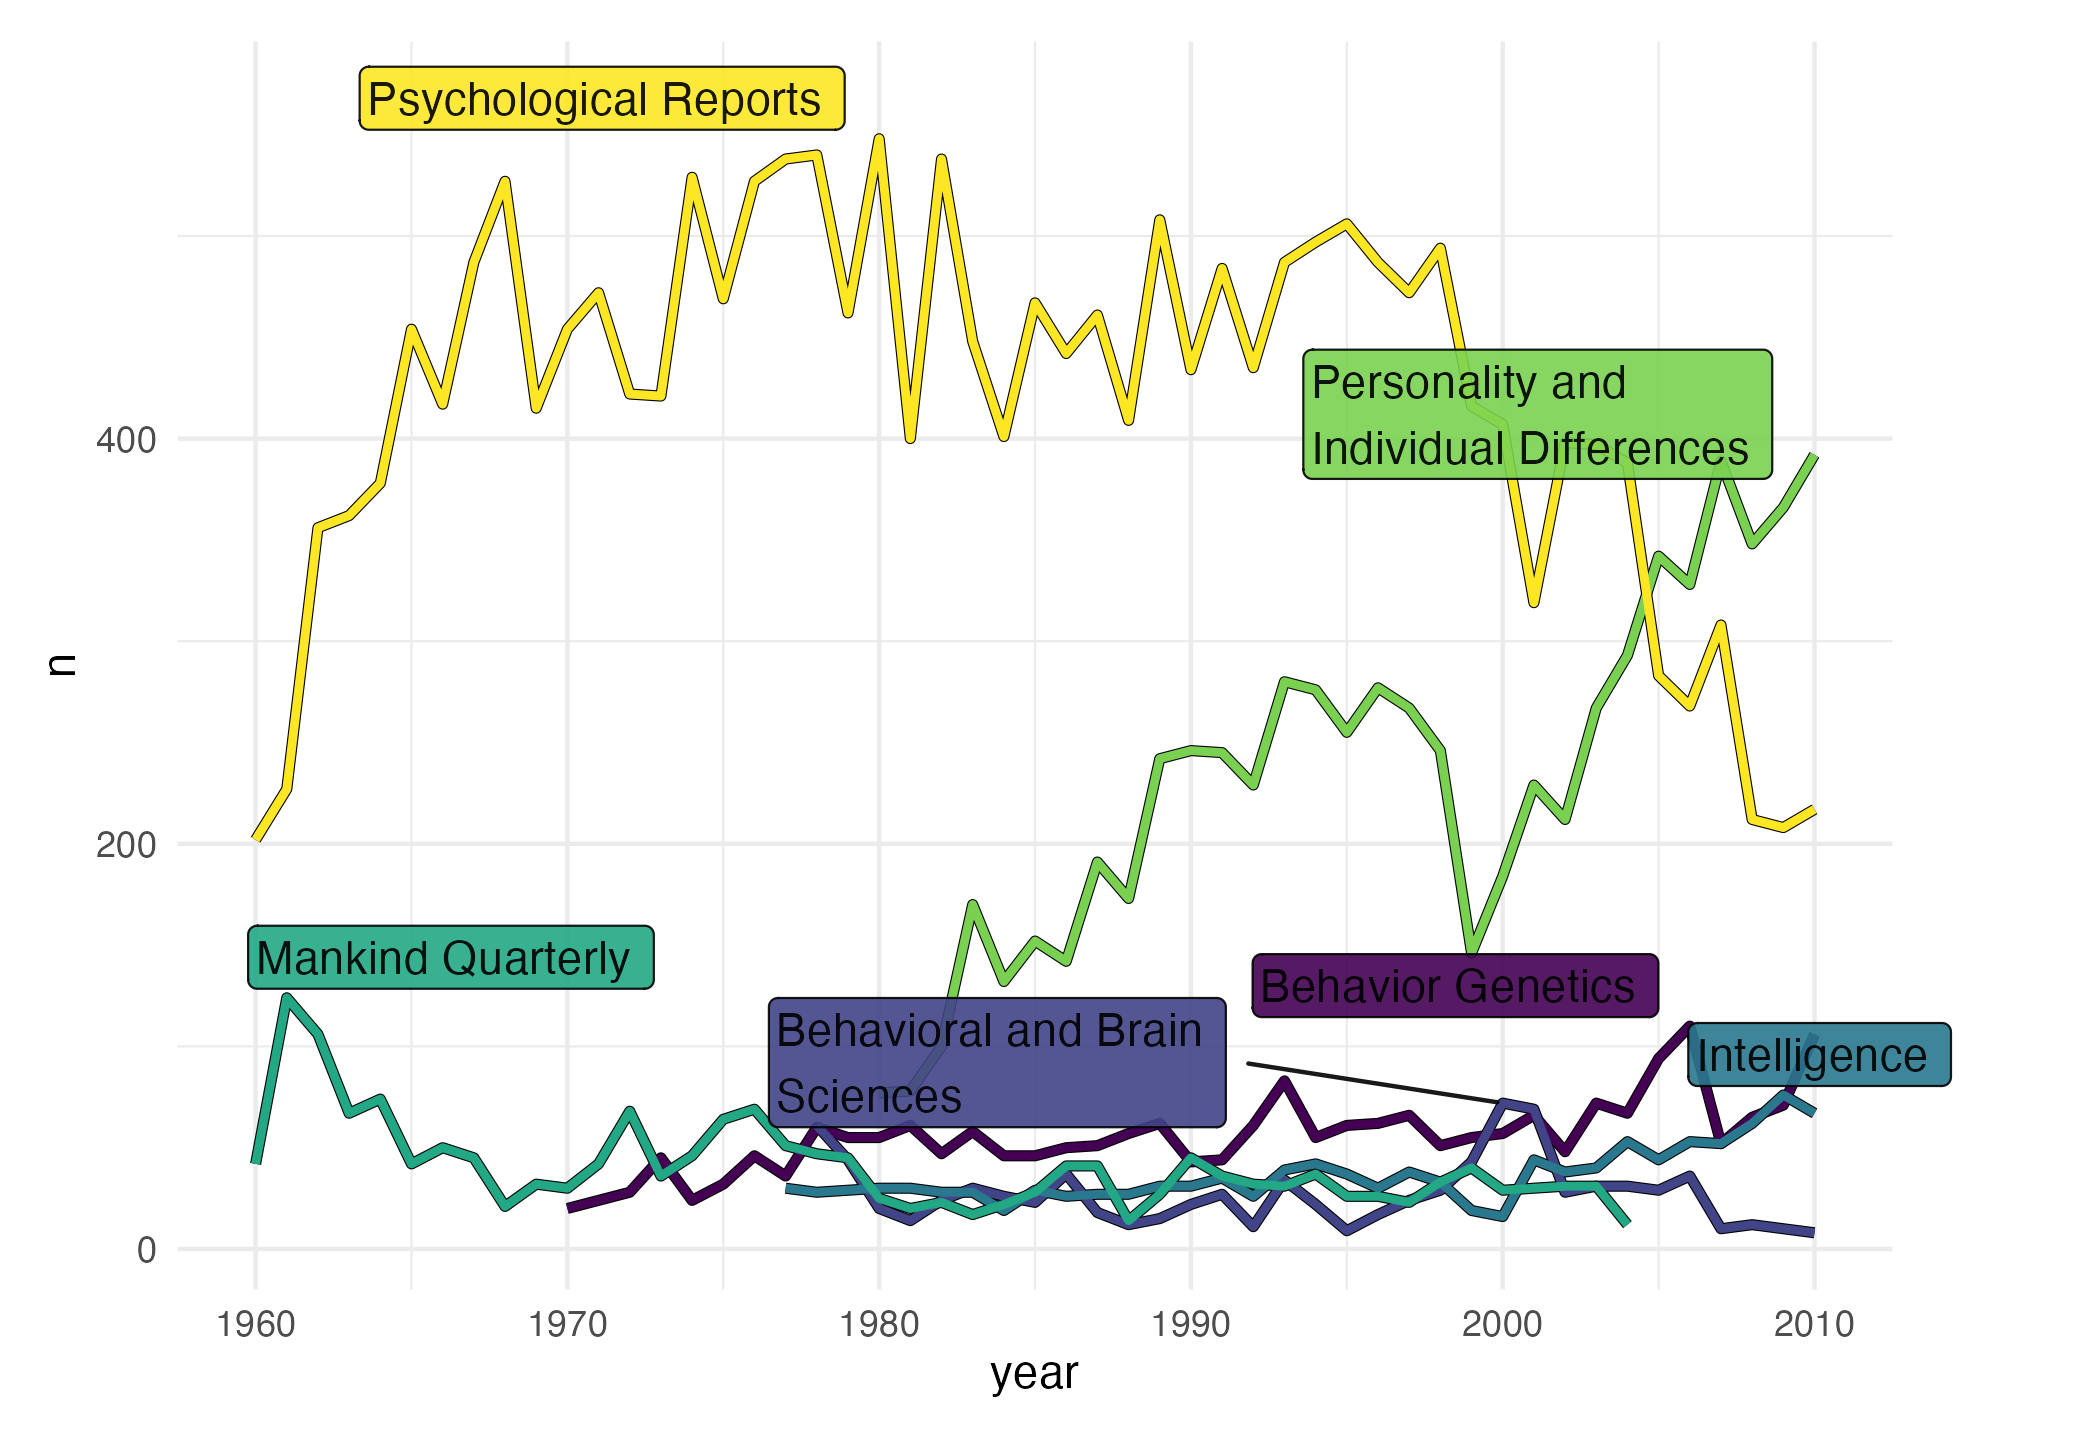
\includegraphics[width=4.76in,height=2.6in]{img/02_count.png}
\caption{Count of documents in the corpus, by journal and year. (\#fig:counts)}
\end{figure}

\begin{longtable}[]{@{}lrrr@{}}
\caption{(\#tab:counts) Document counts, by journal, and years included in the corpus.}\tabularnewline
\toprule
journal & n & start & end \\
\midrule
\endfirsthead
\toprule
journal & n & start & end \\
\midrule
\endhead
Behavior Genetics & 2268 & 1970 & 2010 \\
Intelligence & 1237 & 1977 & 2010 \\
Mankind Quarterly & 1821 & 1960 & 2004 \\
Personality and Individual Differences & 7274 & 1980 & 2010 \\
Psychological Reports & 21398 & 1960 & 2010 \\
Behavioral and Brain Sciences & 898 & 1978 & 2010 \\
\bottomrule
\end{longtable}

All together, the corpus includes 34,896 documents from 6 journals. See @ref(fig:counts) and @ref(tab:counts).

\hypertarget{text-preparation}{%
\subsection*{Text preparation}\label{text-preparation}}

After document retrieval and text extraction, we pre-processed the text using the \texttt{spaCy} NLP (natural language processing) Python library and the R API \texttt{spacyr} \emph{{[}version, cites{]}}. Specifically, we applied regular expressions to remove header/footer copyright notices and hyphenation, used spaCy to annotate and extract noun phrases (eg, ``the intelligence test items''), and then cleaned and standardized these phrases (eg, removing the/an/a, coverting all text to lowercase, and replacing all whitespace with underscores: ``intelligence\_test\_items''). We then counted the occurrence of each noun phrase in the document. The aggregated ``document-term matrix'' was stored in Parquet format \emph{{[}cite{]}} for performance reasons, and written and read using the \texttt{arrow} package for R \emph{{[}cite{]}}. \emph{{[}availability{]}}

NLP-extracted noun phrases offer a number of advantages over the more traditional unigram (``single-word'') tokens. First, noun phrase extraction removes many standard stopwords (articles, common verbs) without relying on a fixed, a priori stopword list. Phrases can be more informative than single terms, for example, distinguishing ``intelligence test'' from ``hypothesis test.'' But simple n-gram extraction will include numerous phrases that are not especially meaningful. Consider the sentence ``Since our first analyses of feeding patterns in rats, we had been using a criterion of 40 minutes (Le Magnen \& Tallon 1963; 1966)'' *{[}10.1017\_\_\^{}\_\_s0140525x0000042x{]}*. Bigrams such as ``since our'' and ``criterion 40'' will likely be discarded in vocabulary selection, but significantly increase the computational cost of vocabulary selection. Noun phrase extraction is therefore more efficient.

After noun phrase extraction, the corpus comprised \emph{{[}tokens{]}} of \emph{{[}distinct noun phrases{]}}.

\hypertarget{data-and-code-availability}{%
\subsubsection*{Data and code availability}\label{data-and-code-availability}}

Document metadata retrieved from Crossref does not appear to be covered by any copyright or other intellectual property restrictions. However, due to copyright restrictions, we are unable to make document fulltext or Web of Science search results publicly available. Code for the corpus assembly and text preparation steps described above is available by request.

The public analysis repository, \url{https://github.com/dhicks/race-science} \emph{{[}DOI{]}}, includes document metadata and documentwise counts of NLP-extracted noun phrases (``document-term matrices''), along with code to reproduce the analysis of the following sections. \emph{{[}repo readme: requires R 4.1.2; rig (\url{https://github.com/r-lib/rig/}) for managing multiple R installations{]}}

\hypertarget{vocabulary-selection}{%
\subsection*{Vocabulary selection}\label{vocabulary-selection}}

We took an information-theoretic approach to vocabulary selection. Consider a game in which I draw a document from the corpus, then a single token from that document. I tell you the term, and you have to guess which document I picked. Intuitively, highly informative terms (in this project, noun phrase types) are distinctive, allowing you to dramatically narrow down the list of potential documents. This ``informativeness'' of a term can be quantified as the KL (Kullback-Leibler) divergence from a ``baseline'' distribution of documents to the distribution conditional on the term. Because the most informative terms tend to be typos and OCR errors --- these are unique to a single document --- we multiply the KL divergence by the logarithm of the total number of occurrences of the term across the entire corpus. We refer to the resulting measure as \(log(n) \Delta H\) or simply \texttt{ndH}.

\emph{{[}Hicks 2021?{]}} used the \texttt{ndH} approach in a topic modeling analysis, where the baseline distribution was the uniform distribution across documents. In the current project, we found that this approach heavily favored recurrent noun phrases in the longest documents. Many of the documents published in \emph{Psychological Reports} are extremely short, 1-2 reports of a single study; while many of the documents published in \emph{Brain and Behavioral Sciences} are book-length collections that include a long review article and sometimes dozens of commentaries. Very generic noun phrases that happen to appear in the latter can occur orders of magnitude more often than highly distinctive phrases in the former, and so the \(log(n)\) factor overwhelms the \(\Delta H\) factor.

To address this, we used a different baseline distribution of documents, namely, one in which document probability is proportional to length. This makes phrases from short documents much more ``surprising'' (much less likely to occur according to the baseline), and hence substantially increases their informativeness. This was more effective at identifying useful phrases from across the corpus.

A common rule of thumb in topic modeling is that the vocabulary should have about 10 times as many distinct terms as the number of documents in the corpus \emph{{[}cite{]}}. However, we had some concerns with computational demands here: the resulting document-term matrix would have roughly \(10 \times 33,000^2\) or 10.9 billion entries; with 10\% density this would require on the order of 4 GB of memory just for a single copy of the matrix; and most of the analysis was to be conducted on the authors' laptops. We therefore chose to work with three smaller vocabularies, \(5 \times\), \(1 \times\) and \(\frac{1/5} \times\) the number of documents. We refer to these as the ``large,'' ``medium,'' and ``small'' vocabulary, respectively, and they include \emph{{[}counts{]}} distinct phrases. We compare findings across vocabularies as a robustness check.

\hypertarget{topic-modeling}{%
\subsection*{Topic modeling}\label{topic-modeling}}

To fit topic models, we followed the approach proposed by \emph{{[}cite{]}}, which uses varimax-rotated partial principal components instead of the variational inference methods used by standard topic model packages \emph{{[}eg, stm{]}}. This novel approach was implemented in the R package \texttt{tmfast}, \emph{{[}cite{]}}. A simulation study of \texttt{tmfast} found that it was significantly faster and only slightly less accurate at reconstructing known word-topic and topic-document distributions, compared to the standard topic modeling package \texttt{stm}.

Topic models were fit for all three vocabularies (large, medium, and small) with \(k = 5, 10, 20, 30, 40, 50\) (number of topics), resulting in a total of 18 models.

Following the approach of \emph{{[}Hicks 2021?{]}}, we did not attempt to identify a unique best model for further analysis. While we focus on the medium vocabulary, \(k=30\) model as the ``median'' among the 18 models fit, we compare and contrast findings from this model with those from the other models.

\hypertarget{topic-model-interpretation}{%
\subsubsection*{Topic model interpretation}\label{topic-model-interpretation}}

After fitting topic models, our first research question was whether we could identify distinctive ``race science'' topics. We addressed this question in two ways. Following common practice in topic modeling, we extracted lists of the top \(n\) (highest-probability) terms (noun phrases) from each topic in each model, with \(n\) generally ranging between 5 and 15 as we explored the models. \emph{{[}tables + Silge plots{]}}

\emph{{[}drop{]}}
We also adapted the ``discursive space'' analysis proposed by \emph{{[}Hicks 2021?{]}}. This analysis combines the Hellinger distance between topic-document distributions --- capturing how ``far apart'' two documents are --- with dimensional reduction techniques used for data visualization. This produces a two-dimensional visualization of individual documents, arranged so that documents with similar topic distributions are visually clustered and visually distinct from documents with different topic distributions. \emph{{[}availability{]}}

Specifically, for each fitted topic model, we extracted topic-document distributions for each document and calculated pairwise Hellinger distances. We then processed these distances using the UMAP algorithm for dimension reduction, as implemented in the \texttt{umap} package \emph{{[}details; cite{]}}. To reduce computational requirements for these steps, we first dropped documents published in the journal \emph{{[}Psychological Reports{]}} (\emph{{[}x documents removed, y remaining{]}}; note that the full corpus was used to fit the topic models, \emph{Psychological Reports} was removed just for this visualization). Using the \texttt{plotly} library \emph{{[}cite{]}}, we construct an interactive visualization: each point represents a single document, and points can be colored based on either their journal or highest-probability topic. Tooltips are displayed when we hover over a point, including document metadata (title, journal, authors, year) as well as ``key phrases.''

To calculate key phrases for a given document \(d\), we first identified the highest-probability topic \(t\) for that document and the word-topic (noun phrase-topic) distribution \(\beta_{w,t}\) for that topic. We also retrieved the document-term matrix, containing the count \(n_{w,d}\) of occurrences for each word (noun phrase), and calculated a weighting \(n_{w,d} \beta_{w,t}\) for each word. The key phrases are the 5 most highly-weighted terms for the given document.

\hypertarget{topic-quality-assessment}{%
\subsubsection*{Topic quality assessment}\label{topic-quality-assessment}}

\emph{{[}rewrite{]}}

We next conducted a topic quality check of topic 19 from the medium vocabulary, \(k=30\) model. Keyword and inspection of the UMAP interactives seemed to indicate that this topic was a ``race science discourse'' topic in this model.

To confirm this initial impression, a spreadsheet of all articles with \(\gamma > 0.25\) for this topic was extracted (excluding articles published in \emph{Psychological Reports}), and the top 200 articles were reviewed manually by both authors. For this qualitative analysis, we defined \emph{scientific racism} as (purporting) to justify racial inequality and colonialism by appealing to the epistemic authority of science; \emph{race science} as (pseudo-)scientific research that can be utilized for scientific racism; and \emph{race science discourse} as treating race science as a legitimate area of scientific research; this includes methodological critiques of race science and empirical tests that falsify race science hypotheses. Our qualitative review of the top-200 topic-19 articles focused on classifying them as \emph{race science discourse}.

For the first round of review, both authors worked independently, dichotomously coding each article as race science discourse or not. We calculated the ``false positive rate'' --- documents with a very high \(\gamma\) in this topic that were not race science discourse --- and interrater reliability using Cohen's \(\kappa\).\\
\emph{{[}false positive rate{]}}
\emph{{[}Initial interrater reliability was low, \(\kappa = 0.4\), with 50 out of 200 articles classified discordantly.{]}} To understand the disagreement, both authors examined the 50 discordant articles using an interactive grounded theory approach. After this process, some initial codings were changed and \emph{{[}almost{]}} all of the remaining \emph{{[}n{]}} discordant articles were coded as follows:

\begin{description}
\tightlist
\item[hereditarianism and/or eugenics]
29 papers. On the ``eugenics'' side, mostly examines or otherwise discusses the ``dysgenic'' claim that ``low-intelligence'' people have more children than ``high-intelligence'' people. The ``hereditarianism'' side is more varied, with papers on environmentalist interventions to raise IQ, genetics of IQ, and several other sub-topics.
\item[Flynn effect]
15 papers. Supporting, challenging, or otherwise focusing on Flynn's findings that IQ has increased over time.
\item[Lynn/national IQ]
3 papers. Supports, challenges, or focuses on international IQ data/comparisons made by Richard Lynn.
\end{description}

We agreed that, for all three categories of papers, there was reasonable ambiguity about whether they should be classified as race science discourse. These papers either do not explicitly mention race, or do so with just a brief mention of the ``race and intelligence controversy.'' On the other hand, they either contribute to or legitimatize areas of research that are deeply entangled with race science, and might thereby contribute to public perceptions of a legitimate scientific debate about race and intelligence.

Based on this qualitative review, we judged that the topic model approach was sufficiently sensitive (low ``false positive'' rate) in identifying race science discourse.

\end{document}
